\documentclass[12pt,preprint]{aastex}

\usepackage{amsmath}

\newcounter{address}
%\newcommand{\latin}[1]{\textit{#1}}
%\newcommand{\cf}{\latin{cf.}}
\newcommand{\eqnnumber}{Equation}
\newcommand{\eqnname}{Equation}
\newcommand{\eg}{e.g.}
\newcommand{\ie}{i.e.}
\newcommand{\Ie}{I.e.}
%\newcommand{\vs}{\latin{vs.}}
\newcommand{\etal}{et~al.}
%\newcommand{\Hipparcos}{\textit{Hipparcos}}
\newcommand{\normal}{{\cal N}}
\newcommand{\wishart}{{\cal W}}
\newcommand{\dirichlet}{{\cal D}}
\renewcommand{\vec}[1]{\mathbf{#1}} % boldface for vectors
\newcommand{\inv}{^{-1}}
\newcommand{\bb}{\vec{b}}
\newcommand{\cc}{\vec{c}}
\newcommand{\ee}{\vec{\hat{e}}}
\newcommand{\mm}{\vec{m}}
\newcommand{\vv}{\vec{v}}
\newcommand{\xx}{\vec{x}}
\newcommand{\zz}{\vec{z}}
\newcommand{\ww}{\vec{w}}
\newcommand{\bij}{\bb_{ij}}
\newcommand{\bbij}{\bij}
%\newcommand{\cci}{\cc_i}
%\newcommand{\eex}{\vec{\hat{x}}}
%\newcommand{\eey}{\vec{\hat{y}}}
%\newcommand{\eez}{\vec{\hat{z}}}
%\newcommand{\eer}{\vec{\hat{r}}_i}
%\newcommand{\eel}{\vec{\hat{l}}_i}
%\newcommand{\eeb}{\vec{\hat{b}}_i}
\newcommand{\mmj}{\mm_j}
\newcommand{\mmk}{\mm_k}
\newcommand{\vvi}{\vv_i}
\newcommand{\vvj}{\vv_j}
%\newcommand{\vvdisk}{\vv_\mathrm{disk}}
%\newcommand{\Kdisk}{K_\mathrm{disk}}
%\newcommand{\vvhalo}{\vv_\mathrm{halo}}
%\newcommand{\vvlsr}{\vv_\mathrm{LSR}}
%\newcommand{\vvsun}{\vv_\odot}
\newcommand{\wwi}{\ww_i}
\newcommand{\wwj}{\ww_j}
\newcommand{\wwk}{\ww_k}
\newcommand{\ten}[1]{\mathbf{#1}} % boldface for tensors
\newcommand{\BB}{\ten{B}}
\newcommand{\CC}{\ten{C}}
\newcommand{\QQ}{\ten{Q}}
\newcommand{\RR}{\ten{R}}
\renewcommand{\SS}{\ten{S}}
\newcommand{\TT}{\ten{T}}
\newcommand{\AAA}{\ten{A}}
\newcommand{\VV}{\ten{V}}
\newcommand{\PP}{\mbox{\bf P}}
\newcommand{\WW}{\ten{W}}
\newcommand{\II}{\ten{I}}
\newcommand{\BBij}{\BB_{ij}}
\newcommand{\CCi}{\CC_i}
\newcommand{\QQi}{\QQ_i}
\newcommand{\RRi}{\RR_i}
\newcommand{\SSi}{\SS_i}
\newcommand{\VVj}{\VV_{\!j}} % \! must be *inside* the subscript, not outside
\newcommand{\VVk}{\VV_{\!k}} % \! must be *inside* the subscript, not outside
%\newcommand{\VVdisk}{\VV_\mathrm{\!disk}}
%\newcommand{\VVhalo}{\VV_\mathrm{\!halo}}
\newcommand{\TTij}{\TT_{ij}}
\newcommand{\TTik}{\TT_{ik}}
\newcommand{\T}{^{\scriptscriptstyle \top}}   % transpose
\newcommand{\iT}{^{\scriptscriptstyle -\top}} % inverse transpose
\newcommand{\tr}{\mathrm{tr}}                 % trace
\newcommand{\alphaj}{\alpha_j}
\newcommand{\alphak}{\alpha_k}
%\newcommand{\alphadisk}{\alpha_\mathrm{disk}}
%\newcommand{\alphahalo}{\alpha_\mathrm{halo}}
\newcommand{\qij}{q_{ij}}
\newcommand{\pij}{p_{ij}}
\newcommand{\pik}{p_{ik}}
\newcommand{\qqj}{q_j}
%\newcommand{\subsamplecolor}{ 0.654<(B-V)< 0.685}
\newcommand{\trace}{\mathrm{Trace}}
\newcommand{\norm}{|\!|}
\newcommand{\MLE}{MLE}
\newcommand{\EPhi}{\langle\Phi\rangle}

\newcommand{\dd}{\textnormal{d}}

\newcommand{\ra}{\ensuremath{\alpha}}
\newcommand{\dec}{\ensuremath{\delta}}
\newcommand{\pmra}{\ensuremath{\mu_{\ra}}}
\newcommand{\pmdec}{\ensuremath{\mu_{\dec}}}
\newcommand{\eqx}{\ensuremath{x_{\textnormal{eq}}}}
\newcommand{\eqy}{\ensuremath{y_{\textnormal{eq}}}}
\newcommand{\eqz}{\ensuremath{z_{\textnormal{eq}}}}
\newcommand{\gall}{{\it l}}
\newcommand{\galb}{{\it b}}
\newcommand{\pmll}{\ensuremath{\mu_\gall}}
\newcommand{\pmbb}{\ensuremath{\mu_\galb}}
\newcommand{\galx}{\ensuremath{x}}
\newcommand{\galy}{\ensuremath{y}}
\newcommand{\galz}{\ensuremath{z}}
\newcommand{\galU}{\ensuremath{U}}
\newcommand{\galV}{\ensuremath{V}}
\newcommand{\galW}{\ensuremath{W}}
\newcommand{\parallax}{\ensuremath{\varpi}}
\newcommand{\radialdist}{\ensuremath{d}}
\newcommand{\vrr}{\ensuremath{v_r}}
\newcommand{\vra}{\ensuremath{v_{\ra}}}
\newcommand{\vdec}{\ensuremath{v_{\dec}}}
\newcommand{\vll}{\ensuremath{v_\gall}}
\newcommand{\vbb}{\ensuremath{v_\galb}}
\newcommand{\vernal}{\ensuremath{\Upsilon}}
\newcommand{\ngp}{\textnormal{NGP}}
\newcommand{\ngpg}{\textnormal{G}}
\newcommand{\ncp}{\textnormal{NCP}}
\newcommand{\ncpp}{\textnormal{P}}
\newcommand{\gc}{\textnormal{GC}}
\newcommand{\gcc}{\textnormal{C}}
\newcommand{\rangp}{\ensuremath{\ra_\ngp}}
\newcommand{\decngp}{\ensuremath{\dec_\ngp}}
\newcommand{\ragc}{\ensuremath{\ra_\gc}}
\newcommand{\decgc}{\ensuremath{\dec_\gc}}
\newcommand{\degree}{^{\circ}}
\newcommand{\matrixleft}{\left[}
\newcommand{\matrixright}{\right]}
\newcommand{\arcsecs}{\textnormal{as}}

\begin{document}

\title{Stellar kinematics}
\author{
  Jo Bovy}

\date{\centering{\it Draft, \today}}

\begin{abstract}
We present the transformations from observed kinematical quantities
(\ra,\dec,\parallax,\pmra,\pmdec) into Galactic quantities
(\galU,\galV,\galW) and (\pmll,\pmbb).
\end{abstract}


\section{From (\ra,\dec) to (\gall,\galb)}

The equatorial coordinates right ascension (\ra) and declination
(\dec) are defined as follows: Consider a very large sphere centered
at the center of the Earth (see \figurename~\ref{fig:eq}). The
intersection of the Earth's axis of rotation with this sphere is
labeled as \ncp\ (which we sometimes abbreviate even further as
\ncpp), the North Celestial Pole. On this sphere there are parallels
and meridians completely analogous to those defined on the surface of
the Earth. Consider a star at a position $X$ on this sphere. The
declination of that star is then defined as the complement of the arc
between \ncp\ and $X$ on the meridian connecting these two points. The
right ascension of the star is defined as the angle between the
meridian through \ncp\ and $X$ and a reference meridian. This
reference meridian is defined as the meridian which intersects the
celestial equator (the intersection of the plane in which the Earth's
equator lies and the celestial sphere) at the point in which the
intersection of the ecliptic, \ie, the plane in which the Earth's
orbit around the Sun lies, with the celestial sphere, the ``celestial
ecliptic`'' if you will, intersects with the celestial equator; this
defines two points, the point chosen is the point at which the Sun
crosses the equatorial plane from South to North. This event is called
the (northern) vernal equinox and it happens around March 21. The
location of the vernal equinox on the celestial sphere is denoted by
\vernal\ \citep[][pp.14-6]{Green85a}. Therefore, \ra\ and \dec\ are
formally defined as
\begin{align}
\dec &= 90\degree - \ncpp X\, ,\\
\ra &= \vernal \ncpp X \, .
\end{align}
Declinations run from $-90\degree$ to $90\degree$ whereas right
ascensions can take on any value between $0\degree$ and $360\degree$.

\begin{figure}[htp]
\begin{center}
\includegraphics[clip=]{radec_fig.eps}
\caption{Definition of the equatorial coordinate system.}\label{fig:eq}
\end{center}
\end{figure}

Galactic coordinates, \ie, a system of coordinates that has the
Galactic plane as its equatorial plane, were introduced as early as
the late eighteenth century by William Herschel and a variety of
definitions existed based mainly on ambiguities in the definition of
the Galactic poles. A standard system was introduced early in the
twentieth century \citep{Ohlsson32a} and the zero of the longitude was
set, rather arbitrarily, at the intersection of the Galactic plane and
the equatorial plane for the equinox 1900.0. After the second World
War, new radio observations revealed that the position of the Galactic
poles needed revision and a new system of Galactic coordinates was
introduced \citep{1960MNRAS.121..123B}. New in this system was that
radio observations had also shown that the compact radio source
Sagittarius A* is at the center of the Galaxy and its position was
used to define the zero of the Galactic longitude.

In detail the Galactic coordinate system is defined as follows (see
\figurename~\ref{fig:lb}): Let \ngp\ be the point on the celestial
sphere corresponding to the North Galactic Pole (we will also
sometimes just call this \ngpg, when brevity is required). The
Galactic latitude \galb\ is the defined as the complement of the arc
along the great circle connecting the star's position $X$ to \ngp. Let
\gc\ be the point on the Galactic equator (that is, the intersection
of the Galactic plane with the celestial sphere) corresponding to the
Galactic center (sometimes simply \gcc). The Galactic longitude
\gall\ of the star $X$ is then the angle on the celestial sphere
between the meridian through the \ngp\ and $X$ and the meridian
through the \ngp\ and the \gc. That is
\begin{align}\label{eq:galcodef}
\galb &= 90\degree - \ngpg X \, ,\\
\gall &= \gcc \ngpg X \, .
\end{align}
Galactic latitudes run from $-90\degree$ to $90\degree$ whereas Galactic
longitudes can take on any value between $0\degree$ and $360\degree$.

To derive the transformation between equatorial coordinates of a star
and the Galactic coordinates we need the coordinates of the \ngp\ and
the \gc\ in the equatorial frame, \ie, we need $\rangp$, $\decngp$,
and the position angle of the Galactic center $\theta$, or
equivalently, the Galactic longitude of the north celestial
pole. These quantities were defined for the epoch 1950.0 as follows:
\citep{1960MNRAS.121..123B}
\begin{align}\label{eq:IAUNGPGC}
\rangp &= 12^{\textnormal{h}}49^{\textnormal{m}} = 192\degree.25\, ,\\
\decngp &= 27\degree.4\, ,\\
\theta &= 123\degree\, .
\end{align}
We also need some formulas from spherical trigonometry, which are
given in the following subsection.

\subsection{Some formulas from spherical trigonometry}

To derive the transformation between equatorial coordinates and
Galactic coordinates we need three formulas from spherical
trigonometry: the cosine formula, the sine formula, and the analogue
formula. Let $ABC$ be a spherical triangle and let $a$ be the arc
between $B$ and $C$ (that is, the arc on the great circle connecting
$B$ and $C$) and analogous for $b$ and $c$. Also let, through a slight
abuse of notation, $A$ be the angle between the meridians on which $B$
respectively $C$ lie, where the meridians are defined with respect to
the pole $A$, and similarly for $B$ and $C$. Then the following holds:
\begin{align}
\sin a \cos B & = \cos b \sin c - \sin b \cos c \cos A\, \qquad \qquad \, \textnormal{(analogue formula)}\,\label{eq:analogue}\\
\frac{\sin A}{\sin a} & = \frac{\sin B}{\sin b} = \frac{\sin C}{\sin c} \ \ \quad\qquad \qquad\qquad \qquad \textnormal{(sine formula)}\,\label{eq:sineform}\\
\cos a &= \cos b \cos c + \sin b \sin c \cos A\qquad \qquad\ \textnormal{(cosine formula)}\label{eq:cosineform}\, .
\end{align}



\subsection{The transformation from (\ra,\dec) to (\gall,\galb)}

\begin{figure}[htp]
\begin{center}
\includegraphics[clip=]{lb_fig.eps}
\caption{Transformation between the equatorial and Galactic coordinate
  systems.}\label{fig:lb}
\end{center}
\end{figure}

We can now derive the transformation from equatorial coordinates to
Galactic coordinates. We will consider the spherical triangle $\ngpg P
X$ on the celestial sphere (see \figurename~\ref{fig:lb}). If the
point $X$ has Galactic coordinates (\gall,\galb) and equatorial
coordinates (\ra,\dec) then we have the following \citep{Green85a}:
\begin{align}\label{eq:triangleGPX}
\ncpp X &= 90\degree-\dec\, ,\\
\ngpg X &= 90\degree - \galb\, ,\\
\ngpg\ncpp &= 90\degree-\decngp\, ,\\
\ngpg \ncpp X &= \ra-\rangp\, ,\\
\ncpp \ngpg X &= \theta-\gall\, .
\end{align}
A simple application of the analogue formula (\ref{eq:analogue}) gives
\begin{equation}
\sin \ngpg X \cos \ncpp \ngpg X = \cos \ncpp X \sin \ngpg \ncpp - \sin \ncpp X \cos \ngpg \ncpp  \cos \ngpg \ncpp X\, .\\
\end{equation}
Substituting in (\ref{eq:triangleGPX}) this becomes
\begin{equation}
\sin(90\degree - \galb) \cos(\theta-\gall) = \cos(90\degree-\dec) \sin(90\degree-\decngp) - \sin(90\degree-\dec) \cos(90\degree-\decngp) \cos(\ra-\rangp)\, ,\\
\end{equation}
which becomes
\begin{equation}\label{eq:radectolb1}
\cos\galb \cos(\theta-\gall) = \sin\dec \cos\decngp - \cos\dec \sin\decngp \cos(\ra-\rangp)\, .
\end{equation}
The sine formula (\ref{eq:sineform}) gives in this case:
\begin{equation}
\frac{\sin \ngpg \ncpp X}{\sin \ngpg X} = \frac{\sin \ncpp \ngpg X}{\sin \ncpp X}\, ,
\end{equation}
and this becomes using (\ref{eq:triangleGPX})
\begin{equation}
\frac{\sin(\ra-\rangp)}{\sin(90\degree - \galb)} = \frac{\sin(\theta-\gall)}{\sin(90\degree-\dec)}\, ,
\end{equation}
which is
\begin{equation}\label{eq:radectolb2}
\cos \galb \sin(\theta-\gall)=\cos \dec \sin (\ra-\rangp)\, .
\end{equation}
And lastly we can apply the cosine formula (\ref{eq:cosineform}) as follows
\begin{equation}
\cos \ngpg X = \cos \ngpg \ncpp  \cos \ncpp X + \sin \ngpg \ncpp \sin \ncpp X \cos \ngpg \ncpp X\, ,
\end{equation}
which becomes using (\ref{eq:triangleGPX})
\begin{equation}
\cos (90\degree - \galb) = \cos(90\degree-\decngp) \cos(90\degree-\dec) + \sin(90\degree-\decngp) \sin(90\degree-\dec) \cos(\ra-\rangp)\, ,
\end{equation}
which simplifies to
\begin{equation}\label{eq:radectolb3}
\sin \galb = \sin \decngp \sin \dec + \cos\decngp \cos\dec \cos(\ra-\rangp)\, .
\end{equation}

The way to use these transformation equations
(\ref{eq:radectolb1}),(\ref{eq:radectolb2}), and (\ref{eq:radectolb3})
is to first use (\ref{eq:radectolb3}) to solve for \galb. Then use
(\ref{eq:radectolb1}) and (\ref{eq:radectolb2}) to unambiguously solve
for \gall.

The transformation given here, using the definitions
(\ref{eq:IAUNGPGC}), is only valid for the epoch 1950.0. We will
describe why this is and how to deal with measurements of
(\ra,\dec) at different epochs below.

\subsubsection{The transformation from (\ra,\dec) to (\gall,\galb) in matrix form}

The transformation equations
(\ref{eq:radectolb1}),(\ref{eq:radectolb2}), and (\ref{eq:radectolb3})
can be written in matrix form which shows that the full transformation
is the combination of three simple transformations. This will also
allow us to easily extract the inverse transformation, i.e~from
(\gall,\galb) to (\ra,\dec).

For convenience we will list the transformation equations
(\ref{eq:radectolb1}),(\ref{eq:radectolb2}), and (\ref{eq:radectolb3}) here together:
\begin{align}\label{eq:radectolb}
\cos\galb \cos(\theta-\gall) &= \sin\dec \cos\decngp - \cos\dec \sin\decngp \cos(\ra-\rangp)\, .\nonumber\\
\cos \galb \sin(\theta-\gall)&= \cos \dec \sin (\ra-\rangp)\, .\nonumber\\
\sin \galb &= \sin \decngp \sin \dec + \cos\decngp \cos\dec \cos(\ra-\rangp)\, .
\end{align}
We will show now that these transformation equations can be written as
\begin{equation}\label{eq:radectolbmatrix}
\matrixleft \begin{array}{c} \cos \galb \cos \gall \\ \cos \galb \sin \gall \\ \sin \galb \end{array} \matrixright =
\TT \matrixleft \begin{array}{c} \cos \dec \cos \ra \\ \cos \dec \sin \ra \\ \sin \dec \end{array} \matrixright\, ,
\end{equation}
where $\TT \equiv \TT(\rangp,\decngp,\theta)$, and thus can be
evaluated for the epoch at which the (\ra,\dec) are measured.

The right hand sides of (\ref{eq:radectolb}) can be written in matrix
form as follows:
\begin{equation}\label{eq:radectolbmatrix1}
\matrixleft \begin{array}{c} \cos \galb \cos (\theta - \gall) \\ \cos \galb \sin(\theta-\gall)\\ \sin \galb \end{array} \matrixright  = 
\matrixleft \begin{array}{ccc} \cos \theta & \sin \theta & 0\\\sin \theta & -\cos \theta & 0\\0&0&1 \end{array} \matrixright
\matrixleft \begin{array}{c} \cos \galb \cos \gall \\ \cos \galb \sin \gall \\ \sin \galb \end{array} \matrixright\, .
\end{equation}
The left hand sides of (\ref{eq:radectolb}) can be similarly be written first as:
\begin{equation}\scriptstyle\label{eq:radectolbmatrix2}
\matrixleft \begin{array}{c} \sin\dec \cos\decngp - \cos\dec \sin\decngp \cos(\ra-\rangp)\\ 
\cos \dec \sin (\ra-\rangp)\\
\sin \decngp \sin \dec + \cos\decngp \cos\dec \cos(\ra-\rangp) \end{array} \matrixright = 
\matrixleft \begin{array}{ccc} -\sin \decngp & 0 & \cos \decngp\\ 0 & 1 & 0 \\ \cos \decngp & 0 & \sin \decngp\end{array} \matrixright 
\matrixleft \begin{array}{c} \cos \dec \cos(\ra - \rangp)\\\cos \dec \sin(\ra-\rangp)\\\sin\dec \end{array} \matrixright\, .
\end{equation}
The final vector in the previous equation can itself be written as
\begin{equation}\label{eq:radectolbmatrix3}
\matrixleft \begin{array}{c} \cos \dec \cos(\ra - \rangp)\\\cos \dec \sin(\ra-\rangp)\\\sin\dec \end{array} \matrixright = 
\matrixleft \begin{array}{ccc} \cos \rangp &\sin\rangp&0\\ -\sin\rangp & \cos\rangp&0\\ 0&0&1\end{array} \matrixright
\matrixleft \begin{array}{c} \cos \dec \cos \ra \\ \cos \dec \sin \ra \\ \sin \dec \end{array} \matrixright\, .
\end{equation}
Combining (\ref{eq:radectolbmatrix1}), (\ref{eq:radectolbmatrix2}), and (\ref{eq:radectolbmatrix3}) we can write
\begin{equation}
\begin{split}
\matrixleft \begin{array}{ccc} \cos \theta & \sin \theta & 0\\\sin \theta & -\cos \theta & 0\\0&0&1 \end{array} \matrixright
\matrixleft \begin{array}{c} \cos \galb \cos \gall \\ \cos \galb \sin \gall \\ \sin \galb \end{array} \matrixright & = 
\matrixleft \begin{array}{ccc} -\sin \decngp & 0 & \cos \decngp\\ 0 & 1 & 0 \\ \cos \decngp & 0 & \sin \decngp\end{array} \matrixright \\
& \times \matrixleft \begin{array}{ccc} \cos \rangp &\sin\rangp&0\\ -\sin\rangp & \cos\rangp&0\\ 0&0&1\end{array} \matrixright
\matrixleft \begin{array}{c} \cos \dec \cos \ra \\ \cos \dec \sin \ra \\ \sin \dec \end{array} \matrixright\, ,
\end{split}
\end{equation}
which means that we can write the matrix $\TT$ in (\ref{eq:radectolbmatrix}) as
\begin{equation}\label{eq:radectolbT}
\TT = \matrixleft \begin{array}{ccc} \cos \theta & \sin \theta & 0\\\sin \theta & -\cos \theta & 0\\0&0&1 \end{array} \matrixright
\matrixleft \begin{array}{ccc} -\sin \decngp & 0 & \cos \decngp\\ 0 & 1 & 0 \\ \cos \decngp & 0 & \sin \decngp\end{array} \matrixright
\matrixleft \begin{array}{ccc} \cos \rangp &\sin\rangp&0\\ -\sin\rangp & \cos\rangp&0\\ 0&0&1\end{array} \matrixright\, ,
\end{equation}
which is slightly different from but agrees with the representation
given by \citet{1987AJ.....93..864J}.

\subsection{The transformation from (\ra,\dec) to (\gall,\galb) for general epochs}

We can evaluate the transformation matrix $\TT$ given in
(\ref{eq:radectolbT}) for the epoch 1950.0 by plugging in the values
for \rangp, \decngp, and $\theta$ from the definition of the Galactic
coordinate system (\ref{eq:galcodef}). In order to evaluate the matrix
$\TT$ for epochs other than 1950.0 one needs to use the values for
\rangp, \decngp, and $\theta$ for that epoch. These values are
different from the 1950.0 values in general because of the effects of
Luni-solar precession, planetary precession and nutation. The
definition of the equatorial coordinate system is fully specified by
the Earth's rotation axis, \ie, the North celestial pole, and the
position of the ecliptic, which together with the equatorial plane
defines the vernal equinox. Therefore, any changes to the orientation
of the Earth's rotation axis or the position of the ecliptic will
change the equatorial coordinates of a star.

Luni-solar precession comes about due to the torque on the Earth's
rotation axis due to the gravitational interaction with the Moon and
the Sun. If the Earth were a perfect sphere, the gravitational
attraction between the Earth, the Moon and the Sun would produce no
such torque, but, mostly due to its axial rotation, the Earth has
developed an equatorial oblateness which violates the perfect
spherical symmetry. The torque resulting from this depends on the
configuration of the three bodies and the changing distances between
them and produces therefore a rather complicated movement. Broadly
this movement can be characterized by a long-term precessional
movement, which is what is meant by Luni-solar precession, of the
Earth's rotation axis, modulated by short-term variations, which is
called the nutation.

The other planets in the Solar system have a negligible influence on
the orientation of the Earth's rotational axis, however, planetary
perturbations do influence the Earth's orbit around the Sun, \ie, they
induce small changes in the orbital elements describing the orbit of
the Earth around the Sun. In particular, the inclination of the
ecliptic is not fixed. This gives rise to the so-called planetary
precession, which corresponds to the change in the equatorial
coordinate system due to the changing inclination of the ecliptic.

In order to derive high precision Galactic coordinates for objects on
the sky, the complicated phenomena of Luni-Solar precession, nutation,
and planetary precession need to be known at a high accuracy and the
corresponding changes to an objects equatorial coordinates need to be
modeled at high accuracy as well. We will not derive these formulas
here, but simply state the result to second order \citep[as given
in][]{Green85a} relative to the epoch J2000.0 (where the ``J''
indicates that this is a Julian date; the epoch 1950.0 is actually
B1950.0, where the ``B'' indicates that this is a Besselian date). To
second order the equatorial coordinates at a time $t$ from J2000.0,
expressed in Julian centuries, are given in terms of those at J2000.0
as follows:
\begin{align}
\ra & = \ra_{\textnormal{J}2000.0} + M + N \sin \ra_m \tan \dec_m\nonumber\\
\dec & = \dec_{\textnormal{J}2000.0} + N \cos \alpha_m\nonumber\\
\ra_m & = \ra_{\textnormal{J}2000.0} +\frac{1}{2} (M + N \sin \ra_{\textnormal{J}2000.0} \tan \dec_{\textnormal{J}2000.0})\label{eq:radecJtoradect}\\
\dec_m & = \dec_{\textnormal{J}2000.0} + \frac{1}{2} N \cos \alpha_m\nonumber\\
M &= 1\degree.281232 \ t + 0\degree.000388 \ t^2\nonumber\\
N &= 0\degree.556753 \ t - 0\degree.000119 \ t^2\, . \nonumber
\end{align}

Given the transformation equations (\ref{eq:radecJtoradect}) we can
evaluate the transformation matrix $\TT$ at any epoch $t$ by
calculating the values of the defining parameters (\ref{eq:galcodef})
at that epoch. The value of $\theta$ at a given epoch can be
calculated from the position of the \ngp\ (\rangp,\decngp) and the \gc\
(\ragc,\decgc) at that epoch. To see how this is done we need to apply
some basic spherical trigonometry again. We consider the spherical
triangle spanned by the \ngp, the \gc, and the \ncp: An application of
the sine rule (\ref{eq:sineform}) gives
\begin{equation}
\frac{\sin \gcc \ngpg \ncpp}{\sin \gcc \ncpp} = \frac{\sin \ngpg \ncpp \gcc}{\sin \ngpg \gcc}\, ,
\end{equation}
or
\begin{equation}
\frac{\sin \theta}{\cos \decgc} = \frac{\sin(\ragc -\rangp)}{\cos \galb_{\gc}}\, ,
\end{equation}
in which $\galb_{\gc} = 0$. Similarly the cosine rule (\ref{eq:cosineform}) gives
\begin{equation}
\cos \gcc \ncpp = \cos \gcc \ngpg \cos \ngpg \ncpp + \sin \gcc \ngpg \sin \ngpg \ncpp \cos \gcc \ngpg \ncpp\, ,
\end{equation}
which becomes
\begin{equation}
\sin \decgc = \sin b_{\gc} \sin \decngp + \cos b_{\gc} \cos \decngp  \cos \theta\, .
\end{equation}
Therefore, we can find $\theta$ by solving the following set of equations
\begin{align}\label{eq:thetafngpgc}
\sin \theta & = \sin(\ragc - \rangp)\cos \decgc\\
\cos \theta &= \frac{\sin \decgc}{\cos\decngp}\, .
\end{align}

The positions of the \ngp\ and the \gc\ for the epoch J2000.0 are
given by \citep[]{1998gaas.book.....B}
\begin{align}
(\rangp,\decngp) & = (192\degree.85948,27\degree.12825)\nonumber\\
(\ragc, \decgc) &= (266\degree.405,-28\degree.936)\, \label{eq:ngpgcJ2000.0}.
\end{align}
From these we can calculate $\theta$ from (\ref{eq:thetafngpgc}) at
epoch J2000.0
\begin{equation}\label{eq:thetaJ2000.0}
\theta = 122\degree.932\, .
\end{equation}

The procedure to transform the position of a star given in (\ra,\dec)
at a given epoch to its Galactic coordinates (\gall,\galb) is now as
follows: First calculate the position of the \ngp\ and the \gc\ in
equatorial coordinates using (\ref{eq:radecJtoradect}) with the values
given in (\ref{eq:ngpgcJ2000.0}); then use (\ref{eq:thetafngpgc}) to
calculate the position angle of the \gc\ for the given epoch; finally
evaluate the transformation matrix $\TT$ (\ref{eq:radectolbT}) for the
calculated values (\rangp,\decngp,$\theta$) and apply this
transformation as in (\ref{eq:radectolbmatrix}).


\section{Parallax}

The annual motion of the Earth around the Sun gives rise to an
apparent displacement of a star relative to background objects that is
inversely proportional to the distance to the star. Measurements of
this apparent shift, or parallax, can thus be used to determine the
distance to stars. Parallaxes are traditionally reported in units of
arcseconds; a star with a parallax of 1 arcsecond is defined to be at
a distance of 1 parsec (pc), which is approximately $3\times 10^{16}$
m. The intrinsic motion of a star also gives rise to a systematic
shift in its position relative to background sources, such that its
angular motion---known as its proper motion---can be
measured. Combining the distance and angular velocity gives the
components of the space velocity of a star that are perpendicular to
the line of sight.

When all three position coordinates of an object are known, \ie, its
position on the celestial sphere and the radial distance
1/\parallax\ to it, its position can be specified in a rectangular
coordinate system. We consider the following two rectangular
coordinate systems: (1) the rectangular equatorial coordinate system
and (2) the rectangular Galactic coordinate system. The rectangular
equatorial coordinate system is defined as follows: the \eqz-axis is
the axis that goes from the center of the celestial sphere to the
\ncp; the \eqx-axis goes from the center to the vernal equinox
\vernal; and the \eqy-axis completes the set such that the coordinate
system is an orthogonal, right-handed system. The rectangular
equatorial coordinates of a star are then given in terms of
(1/\parallax,\ra,\dec) as:
\begin{align}\label{eq:receq}
\eqx &= \frac{1}{\parallax} \cos \dec \cos \ra\, ,\\
\eqy &= \frac{1}{\parallax} \cos \dec \sin \ra\, ,\\
\eqz &= \frac{1}{\parallax} \sin \dec\, .
\end{align}

The rectangular Galactic coordinate system, which is more useful for
studies of the dynamics in the Solar neighborhood, is similarly
defined as follows: the \galz-axis is defined as the axis that goes
from the center of the celestial sphere to the \ngp; the \galx-axis is
defined as the axis from the center to the \gc; the \galy-axis which
completes this set to form a right-handed set is in the direction of
the Galactic rotation. The rectangular Galactic coordinates of a star
are then given by
\begin{align}\label{eq:recgal}
\galx &= \frac{1}{\parallax} \cos \galb \cos \gall\, ,\\
\galy &= \frac{1}{\parallax} \cos \galb \sin \gall\, ,\\
\galz &= \frac{1}{\parallax} \sin \galb\, .
\end{align}


\section{From (\vrr,\pmra,\pmdec) to (U,V,W) and to (\vrr,\pmll,\pmbb)}

We will now describe the transformation of the observed motion of a
star to the motion of the star in the rectangular Galactic coordinate
system. The velocity of a star in the rectangular Galactic coordinate
system is conventially denoted as
\begin{equation}
(\galU,\galV,\galW) \equiv (\dot{\galx},\dot{\galy},\dot{\galz})\, .
\end{equation}
Since observations of the movement of a star are generally done by
comparing the (\ra,\dec) of the star at different epochs, while
measurements of its motion in the radial direction are done using the
Doppler shift displayed in the star's spectrum, which measures the
change in the distance \radialdist = 1/\parallax\ directly, we will
relate the velocity components \galU, \galV, and \galW\ to the changes
$\dot{d} \equiv \vrr$, $\dot{\ra}$, and $\dot{\dec}$. In the following
we will be dealing with the distance \radialdist, with the tacit
assumption that actual distances are measured as inverse parallaxes,
while changes in distances are directly measured.

The transformation between the rectangular equatorial coordinate
system and the rectangular Galactic coordinate system is given similar
to (\ref{eq:radectolbmatrix}) as
\begin{equation}\label{eq:receqtorecgal}
\matrixleft \begin{array}{c} \galx \\ \galy \\ \galz \end{array} \matrixright =
\TT \matrixleft \begin{array}{c} \eqx \\ \eqy \\ \eqz \end{array} \matrixright\, ,
\end{equation}
in which $\TT$ is the same transformation matrix as given in
(\ref{eq:radectolbT}). Since the matrix $\TT$ is constant, we can
write
\begin{equation}
\matrixleft \begin{array}{c} \galU \\ \galV \\ \galW \end{array} \matrixright =
\TT\,  \frac{\dd}{\dd t} \matrixleft  \begin{array}{c} \eqx \\ \eqy \\ \eqz \end{array} \matrixright\, ,
\end{equation}
or
\begin{equation}
\matrixleft \begin{array}{c} \galU \\ \galV \\ \galW \end{array} \matrixright =
\TT\,  \frac{\dd}{\dd t} \matrixleft  \begin{array}{c} \radialdist \cos \dec \cos \ra \\ \radialdist \cos \dec \sin \ra \\ \radialdist \sin \dec \end{array} \matrixright\, ,
\end{equation}
which becomes
\begin{equation}\label{eq:simplifyddtradec1}
\matrixleft \begin{array}{c} \galU \\ \galV \\ \galW \end{array} \matrixright =
\TT\, \matrixleft  \begin{array}{c} 
\cos \dec \cos \ra\, \dot{\radialdist} - \radialdist \sin \dec \cos \ra\, \dot{\dec} - \radialdist \cos \dec \sin \ra\, \dot{\ra}
\\ \cos \dec \sin \ra\, \dot{\radialdist} - \radialdist \sin \dec \sin \ra\, \dot{\dec} + \radialdist \cos \dec \cos \ra\, \dot{\ra} 
\\ \sin \dec\, \dot{\radialdist} + \radialdist \cos \dec\, \dot{\dec} \end{array} \matrixright\, .
\end{equation}
This can be simplified by writing
\begin{equation}\label{eq:simplifyddtradec2}
\matrixleft  \begin{array}{c} 
\cos \dec \cos \ra\, \dot{\radialdist} - \radialdist \sin \dec \cos \ra\, \dot{\dec} - \radialdist \cos \dec \sin \ra\, \dot{\ra}
\\ \cos \dec \sin \ra\, \dot{\radialdist} - \radialdist \sin \dec \sin \ra\, \dot{\dec} + \radialdist \cos \dec \cos \ra\, \dot{\ra} 
\\ \sin \dec\, \dot{\radialdist} + \radialdist \cos \dec\, \dot{\dec} \end{array} \matrixright= 
\matrixleft \begin{array}{ccc} \cos \ra & -\sin \ra & 0 \\ \sin \ra & \cos \ra & 0 \\ 0 & 0& 1 \end{array} \matrixright
\matrixleft \begin{array}{c} \cos \dec \, \dot{\radialdist} - \radialdist \sin \dec \, \dot{\dec} \\
\radialdist \cos \dec\, \dot{\ra}\\
\sin\dec \, \dot{\radialdist} + \radialdist \cos\dec\, \dot{\dec} \end{array} \matrixright \, ,
\end{equation}
which can be further simplified as
\begin{equation}\scriptstyle\label{eq:simplifyddtradec3}
\matrixleft  \begin{array}{c} 
\cos \dec \cos \ra\, \dot{\radialdist} - \radialdist \sin \dec \cos \ra\, \dot{\dec} - \radialdist \cos \dec \sin \ra\, \dot{\ra}
\\ \cos \dec \sin \ra\, \dot{\radialdist} - \radialdist \sin \dec \sin \ra\, \dot{\dec} + \radialdist \cos \dec \cos \ra\, \dot{\ra} 
\\ \sin \dec\, \dot{\radialdist} + \radialdist \cos \dec\, \dot{\dec} \end{array} \matrixright= 
\matrixleft \begin{array}{ccc} \cos \ra & -\sin \ra & 0 \\ \sin \ra & \cos \ra & 0 \\ 0 & 0 & 1 \end{array} \matrixright
\matrixleft \begin{array}{ccc} \cos \dec & 0 & \sin \dec\\ 0 & 1 & 0 \\ \sin \dec  & 0 & \cos\dec\end{array} \matrixright
\matrixleft \begin{array}{c} \dot{\radialdist} \\ \radialdist\,\dot{\ra}\,\cos\dec\\\radialdist\dot{\dec}\end{array} \matrixright\, .
\end{equation}
We define
\begin{equation}
\AAA \equiv \matrixleft \begin{array}{ccc} \cos \ra & -\sin \ra & 0 \\ \sin \ra & \cos \ra & 0 \\ 0 & 0& 1 \end{array} \matrixright
\matrixleft \begin{array}{ccc} \cos \dec & 0 & -\sin \dec\\ 0 & 1 & 0 \\ \sin \dec  & 0 & \cos\dec\end{array} \matrixright\, ,
\end{equation}
such that we can write
\begin{equation}\label{eq:vrpmrapmdectoUVW1}
\matrixleft \begin{array}{c} \galU \\ \galV \\ \galW \end{array} \matrixright =
\TT \, \AAA \, \matrixleft \begin{array}{c} \vrr  \\ \frac{1}{\parallax}\,\dot{\ra}\,\cos\dec\\\frac{1}{\parallax}\dot{\dec}\end{array} \matrixright\, .
\end{equation}
Here we used the fact that $\dot{\radialdist} \equiv \vrr$. Note that
the matrix $\AAA$ depends on the position of the star, that is $\AAA
\equiv \AAA(\ra,\dec)$. Let us define $\pmra \equiv \dot{\ra}$ and
$\pmdec \equiv \dot{\dec}$. Generally, the proper motions reported in
astrometrical catalogues are such that $\pmra$ has already been
multiplied with the $\cos \dec$ factor which features in
(\ref{eq:vrpmrapmdectoUVW1}).

Assuming that parallaxes are given in units of arcseconds (\arcsecs),
such that the distance is given in parsec, and that proper motions are
given in units of \arcsecs\ yr$^{-1}$, we need a constant of
proportionality in the transformation (\ref{eq:vrpmrapmdectoUVW1}) if
we want (\galU,\galV,\galW) in units of km s$^{-1}$. We have that
\begin{align}
1 \, \arcsecs &= \frac{\pi}{180 \times 3600} \textnormal{  rad}\,\\[10pt]
1 \textnormal{ pc} &= \frac{180 \times 3600}{\pi} \textnormal{  AU}\, ,
\end{align}
where AU is one astronomical unit. Therefore the constant of
proportionality is given by $k = 1 $AU yr$^{-1}$ expressed in units of km s$^{-1}$. The year here is the tropical year, and we have
\begin{equation}
\textnormal{Tropical year } = 365.242198 \textnormal{ days}\, ,
\end{equation}
such that
\begin{equation}
k = 4.74047\, .
\end{equation}
Therefore, we summarize
\begin{equation}\label{eq:vrpmrapmdectoUVW2}
\matrixleft \begin{array}{c} \galU \\ \galV \\ \galW \end{array} \matrixright =
\TT \, \AAA \, \matrixleft \begin{array}{c} \vrr  \\ \frac{k}{\parallax}\,\pmra\,\cos\dec\\\frac{k}{\parallax}\pmdec\end{array} \matrixright\, ,
\end{equation}
where [\vrr] = km s$^{-1}$, [\parallax] = \arcsecs, and [\pmra]=[\pmdec]= \arcsecs\ yr$^{-1}$.


To go to a description of the motion in terms of proper motions in the
Galactic coordinates we can go through a similar argument as the one
used in (\ref{eq:simplifyddtradec1})-(\ref{eq:simplifyddtradec3}) and
write
\begin{equation}
\matrixleft \begin{array}{c} \galU \\ \galV \\ \galW \end{array} \matrixright =
\matrixleft \begin{array}{ccc} \cos \gall & -\sin \gall & 0 \\ \sin \gall & \cos \gall & 0 \\ 0 & 0 & 1 \end{array} \matrixright
\matrixleft \begin{array}{ccc} \cos \galb & 0 & \sin \galb\\ 0 & 1 & 0 \\ \sin \galb  & 0 & \cos\galb\end{array} \matrixright
\matrixleft \begin{array}{c} \dot{\radialdist} \\ \radialdist\,\dot{\gall}\,\cos\galb\\\radialdist\dot{\galb}\end{array} \matrixright\, .
\end{equation}
We define
\begin{equation}
\RR\T \equiv \matrixleft \begin{array}{ccc} \cos \gall & -\sin \gall & 0 \\ \sin \gall & \cos \gall & 0 \\ 0 & 0 & 1 \end{array} \matrixright
\matrixleft \begin{array}{ccc} \cos \galb & 0 & -\sin \galb\\ 0 & 1 & 0 \\ \sin \galb  & 0 & \cos\galb\end{array} \matrixright\, ,
\end{equation}
$\dot{\gall} \equiv \pmll$, and $\dot{\galb} \equiv \pmbb$, such that
\begin{equation}\label{eq:vrpmllpmbbtoUVW}
\matrixleft \begin{array}{c} \vrr  \\ \frac{k}{\parallax}\,\pmll\,\cos\galb\\\frac{k}{\parallax}\pmbb\end{array} \matrixright = 
\RR \matrixleft \begin{array}{c} \galU \\ \galV \\ \galW \end{array} \matrixright\, ,
\end{equation}
where we have included the $k$ factor defined above to allow
parallaxes and proper motions to be specified in \arcsecs\ and
\arcsecs\ yr$^{-1}$, repectively. Defining $\vll \equiv
\frac{k}{\parallax}\,\pmll\,\cos\galb$ and $\vbb \equiv
\frac{k}{\parallax}\pmbb$ this becomes
\begin{equation}\label{eq:UVWtovrvlvb1}
\matrixleft \begin{array}{c} \vrr  \\ \vll\\\vbb\end{array} \matrixright = 
\RR \matrixleft \begin{array}{c} \galU \\ \galV \\ \galW \end{array} \matrixright\, .
\end{equation}
The full transformation from (\vrr,\pmra,\pmdec) to (\vrr,\vll,\vbb)
can then be written by combining (\ref{eq:vrpmrapmdectoUVW2}) and
(\ref{eq:UVWtovrvlvb1}), such that
\begin{equation}\label{eq:UVWtovrvlvb2}
\matrixleft \begin{array}{c} \vrr  \\ \vll\\\vbb\end{array} \matrixright = 
\RR \, \TT \, \AAA \, \matrixleft \begin{array}{c} \vrr  \\ \frac{1}{\parallax}\,\pmra\,\cos\dec\\\frac{1}{\parallax}\pmdec\end{array} \matrixright\, .
\end{equation}


\subsection{Straight from (\pmra,\pmdec) to (\pmll,\pmbb)}\label{sec:pmtrans}

\eqnnumber~(\ref{eq:UVWtovrvlvb2}) can be simplified to a single
rotation such that
\begin{equation}
\matrixleft \begin{array}{c} \vrr  \\ \frac{1}{\parallax}\,\pmll\,\cos\galb\\\frac{1}{\parallax}\pmbb\end{array} \matrixright = 
\matrixleft \begin{array}{ccc} 1 & 0 & 0 \\ 0 & \cos \phi & \sin \phi \\ 0 & -\sin\phi & \cos\phi\end{array} \matrixright \,\matrixleft \begin{array}{c} \vrr  \\ \frac{1}{\parallax}\,\pmra\,\cos\dec\\\frac{1}{\parallax}\pmdec\end{array} \matrixright
\, .
\end{equation}
One can show by working out the matrix product $\RR\,\TT\,\AAA$ and
using the identities from \eqnnumber~(\ref{eq:radectolb}) that the
\emph{Galactic parallactic angle} $\phi$ is the solution of
\begin{eqnarray}
\cos \phi &=& \frac{\sin \decngp - \sin\dec\sin\galb}{\cos\dec\cos\galb}\, ,\\
\sin \phi &=& \frac{\sin(\ra-\rangp )\cos\decngp}{\cos\galb}\, .
\end{eqnarray}

Therefore, one can directly transform measured proper motions in
celestial coordinates into proper motions in Galactic coordinates as
\begin{equation}\label{eq:pmtrans}
\matrixleft \begin{array}{c} \pmll\,\cos\galb\\\pmbb\end{array} \matrixright = 
\matrixleft \begin{array}{cc} \cos \phi & \sin \phi \\ -\sin\phi & \cos\phi\end{array} \matrixright \,\matrixleft \begin{array}{c} \pmra\,\cos\dec\\\pmdec\end{array} \matrixright
\, .
\end{equation}
We will denote the transformation matrix in this \eqnname\ as \PP.


\section{Uncertainty propagation}\label{sec:errorprop}

Propagation of observational uncertainties is simple using the matrix
formalism employed above. We assume that uncertainties in the
direction $(\ra,\dec)$ of an object are negligible, but we make no
other assumptions about the independence of the uncertainties of the
other quantities since for example the scanning strategy of
astrometric satellites can give rise to correlated proper motion
measurements.

In what follows we give formulas for first-order uncertainty
propagation. We assume that we know the distance uncertainty
$\sigma_d$. If the distance is measured as a parallax, this distance
uncertainty is given by $\sigma_d =
\sigma_\parallax/\parallax^2$. Proper accounting for the non-linear
nature of the transformations above should go beyond this first-order
calculation or employ a Monte Carlo uncertainty propagation.

\subsection{Cov($d$,\vrr,\pmra,\pmdec) to Cov(\galU,\galV,\galW)}

The propagation of uncertainty Cov($d$,\vrr,\pmra,\pmdec) to
Cov(\galU,\galV,\galW) can be broken up into two parts: (i)
Cov($d$,\pmra,\pmdec) to Cov(\vra,\vdec) and (ii) Cov(\vrr,\vra,\vdec)
to Cov(\galU,\galV,\galW), where $\vra \equiv
\frac{k}{\parallax}\,\pmra\,\cos\dec$ and $\vdec \equiv
\frac{k}{\parallax}\pmdec$.

The transformation (i) is non-linear, so we compute the Jacobian as
\begin{equation}
\frac{\partial \left(\vra,\vdec\right)}{\partial\left(d,\pmra,\pmdec\right)}
= k\,\matrixleft \begin{array}{ccc} \pmra \cos \dec & d & 0\\\pmdec & 0 & d\end{array} \matrixright \,.
\end{equation}
Then we have that
\begin{equation}
\mathrm{Cov}(\vra,\vdec) = \frac{\partial \left(
  \vra,\vdec\right)}{\partial \left(d,\pmra,\pmdec\right)}
\mathrm{Cov}(d,\pmra,\pmdec) \frac{\partial \left(
  \vra,\vdec\right)}{\partial \left(d,\pmra,\pmdec\right)}\T\,.
\end{equation}

The transformation (ii) is given by
\eqnname~(\ref{eq:vrpmrapmdectoUVW1}) such that we find
\begin{equation}
\mathrm{Cov}(\galU,\galV,\galW) = \TT\,\AAA \, \mathrm{Cov}(\vrr,\vra,\vdec) \, \AAA\T\,\TT\T\,.
\end{equation}

\subsection{Cov($d$,\vrr,\pmll,\pmbb) to Cov(\galU,\galV,\galW)}

This uncertainty propagation is similar to that in the \sectionname\ above. We again split the transformation into (i) Cov($d$,\pmll,\pmbb) to Cov(\vll,\vbb) and (ii) Cov(\vrr,\vll,\vbb) to Cov(\galU,\galV,\galW), where $\vll \equiv
\frac{k}{\parallax}\,\pmll\,\cos\galb$ and $\vbb \equiv \frac{k}{\parallax}\pmbb$.

The transformation (i) is non-linear with Jacobian
\begin{equation}
\frac{\partial \left(\vll,\vbb\right)}{\partial\left(d,\pmll,\pmbb\right)}
= k\,\matrixleft \begin{array}{ccc} \pmll \cos \galb & d & 0\\\pmbb & 0 & d\end{array} \matrixright \,.
\end{equation}
Then we have that
\begin{equation}
\mathrm{Cov}(\vll,\vbb) = \frac{\partial \left(
  \vll,\vbb\right)}{\partial \left(d,\pmll,\pmbb\right)}
\mathrm{Cov}(d,\pmll,\pmbb) \frac{\partial \left(
  \vll,\vbb\right)}{\partial \left(d,\pmll,\pmbb\right)}\T\,.
\end{equation}

The transformation (ii) is given by
\eqnname~(\ref{eq:UVWtovrvlvb1}) such that we find
\begin{equation}
\mathrm{Cov}(\galU,\galV,\galW) = \RR^{-1}\, \mathrm{Cov}(\vrr,\vll,\vbb) \, \RR\iT\,.
\end{equation}

\subsection{Cov(\pmra,\pmdec) to Cov(\pmll,\pmbb)}

To propagate the proper motion uncertainty in \ra\ and \dec\ to that
in Galactic coordinates (see \sectionname~\ref{sec:pmtrans}) we do
\begin{equation}
\mathrm{Cov}(\pmll \cos \galb,\pmbb) = \PP\, \mathrm{Cov}(\pmra \cos \dec ,\pmdec) \,\PP\T\,,
\end{equation}
where \PP\ is defined below \eqnname~\ref{eq:pmtrans}.








\begin{thebibliography}{5}
\expandafter\ifx\csname natexlab\endcsname\relax\def\natexlab#1{#1}\fi

\bibitem[{{Binney} \& {Merrifield}(1998)}]{1998gaas.book.....B}
{Binney}, J. \& {Merrifield}, M. 1998, {Galactic Astronomy} (Princeton
  University Press)

\bibitem[{{Blaauw} {et~al.}(1960){Blaauw}, {Gum}, {Pawsey}, \&
  {Westerhout}}]{1960MNRAS.121..123B}
{Blaauw}, A., {Gum}, C.~S., {Pawsey}, J.~L., \& {Westerhout}, G. 1960, \mnras,
  121, 123

\bibitem[{{Green}(1985)}]{Green85a}
{Green}, R.~M. 1985, {Spherical astronomy} (Cambridge University Press)

\bibitem[{{Johnson} \& {Soderblom}(1987)}]{1987AJ.....93..864J}
{Johnson}, D.~R.~H. \& {Soderblom}, D.~R. 1987, \aj, 93, 864

\bibitem[{{Ohlsson}(1932)}]{Ohlsson32a}
{Ohlsson}, J. 1932, Ann.~Lund Obs., 6

\end{thebibliography}

\end{document}

